\begin{tabular}{cccc}
% Structure A - Star
\hspace{0.8cm} 
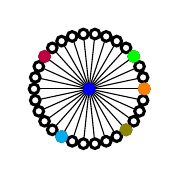
\begin{tikzpicture}[every node/.style={circle, draw, inner sep=2pt, minimum size=6mm}, scale = 0.35, transform shape]
    \tikzstyle{vertex}=[circle, draw = black,fill=White,minimum size=10pt,inner sep=0pt, line width = 1.1pt]
    
    \foreach \label in {2,3,4,5,6,7,8,9}
    {
    \draw  (0,0) -- ({(\label-2)*12}:2cm);
    \node[vertex] (\label) at ({(\label-2)*12}:2cm) {\makebox[0.35cm][c]{\makebox[0.35cm][c]{}}};
    }
    \foreach \label in {10,11,12,13,14,15,16,17,18,19,20,21,22,23,24,25,26,27,28,29,30,31}
    {
    \draw  (0,0) -- ({(\label-2)*12}:2cm);
    \node[vertex] (\label) at ({(\label-2)*12}:2cm) {\makebox[0.35cm][c]{}};
    }
    \node[vertex, fill = blue, draw = blue] (base) at (0,0) {};
    \node[vertex, fill = orange, draw = orange] (base) at (2) {};
    \node[vertex, fill = green, draw = green] (base) at (5) {};
    \node[vertex, fill = purple, draw = purple] (base) at (14) {};
    \node[vertex, fill = cyan, draw = cyan] (base) at (22) {};
    \node[vertex, fill = olive, draw = olive] (base) at (28) {};
    
\end{tikzpicture} &
\hspace{0.6cm}
% Structure B - 5-nary tree
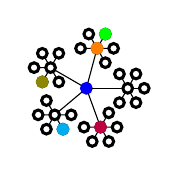
\begin{tikzpicture}[every node/.style={circle, draw, inner sep=2pt, minimum size=6mm}, scale = 0.35, transform shape]
    \tikzstyle{vertex}=[circle, draw = black,fill=White,minimum size=10pt,inner sep=0pt, line width = 1.1pt]
    
    \node[vertex, draw = blue, fill = blue] (base) at (0,0) {};
    
    \foreach \labelngle/\label in {75/2, 360/8, 290/14, 220/20, 150/26}{
        \node[vertex] (noeud\label) at (\labelngle:1.5cm) {\makebox[0.35cm][c]{}};
        \draw (base) -- (noeud\label);
    }
    
    \foreach \labelngle/\label in {360/4, 60/5, 120/6, 180/7, 300/3}{
        \node[vertex] (noeud\label) at ([shift={(\labelngle:0.6cm)}]noeud2) {\makebox[0.35cm][c]{}};
        \draw (noeud2) -- (noeud\label);
    }
    
    \foreach \labelngle/\label in {360/10, 60/11, 120/12, 240/13, 300/9}{
        \node[vertex] (noeud\label) at ([shift={(\labelngle:0.6cm)}]noeud8) {\makebox[0.35cm][c]{}};
        \draw (noeud8) -- (noeud\label);
    }
    
    \foreach \labelngle/\label in {60/15, 360/16, 300/17, 240/18, 180/19}{
        \node[vertex] (noeud\label) at ([shift={(\labelngle:0.6cm)}]noeud14) {\makebox[0.35cm][c]{}};
        \draw (noeud14) -- (noeud\label);
    }
    
    \foreach \labelngle/\label in {360/21, 300/22, 240/23, 180/24, 120/25}{
        \node[vertex] (noeud\label) at ([shift={(\labelngle:0.6cm)}]noeud20) {\makebox[0.35cm][c]{}};
        \draw (noeud20) -- (noeud\label);
    }
    
    \foreach \labelngle/\label in {180/29, 60/31, 120/30, 240/28, 300/27}{
        \node[vertex] (noeud\label) at ([shift={(\labelngle:0.6cm)}]noeud26) {\makebox[0.35cm][c]{}};
        \draw (noeud26) -- (noeud\label);
    }

    \node[vertex, fill = orange, draw = orange]  at (noeud2) {};
    \node[vertex, fill = green, draw = green]  at (noeud5) {};
    \node[vertex, fill = purple, draw = purple]  at (noeud14) {};
    \node[vertex, fill = cyan, draw = cyan]  at (noeud22) {};
    \node[vertex, fill = olive, draw = olive]  at (noeud28) {};
\end{tikzpicture} &
\hspace{0.2cm}
% Structure C - Binary tree
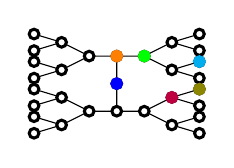
\begin{tikzpicture}[every node/.style={circle, draw, inner sep=2pt, minimum size=6mm}, scale = 0.35, transform shape]
    \tikzstyle{vertex}=[circle, draw = black,fill=White,minimum size=10pt,inner sep=0pt, line width = 1.1pt]
    
    \foreach \label/\x/\y in  {1/3/3.5, 2/3/4.5, 3/3/2.5, 4/2/4.5, 5/4/4.5, 6/2/2.5, 7/4/2.5, 8/1/5, 9/1/4, 10/5/5, 11/5/4, 12/1/3, 13/1/2, 14/5/3, 15/5/2, 16/0/5.3, 17/0/4.7, 18/0/4.3, 19/0/3.7, 20/6/5.3, 21/6/4.7, 22/6/4.3, 23/6/3.7, 24/0/3.3, 25/0/2.7, 26/0/2.3, 27/0/1.7, 28/6/3.3, 29/6/2.7, 30/6/2.3, 31/6/1.7}
    \node[vertex] (G-\label) at (\x,\y){\makebox[0.35cm][c]{}};
    
    \foreach \from/\to in {1/2, 1/3, 2/4, 2/5, 3/6, 3/7, 4/8, 4/9, 5/10, 5/11, 6/12, 6/13, 7/14, 7/15, 8/16, 8/17, 9/18, 9/19, 10/20, 10/21, 11/22, 11/23, 12/24, 12/25, 13/26, 13/27, 14/28, 14/29, 15/30, 15/31}
    \draw (G-\from) -- (G-\to) ;
    \node[vertex, fill = blue, draw = blue] at (G-1) {};
    \node[vertex, fill = orange, draw = orange] at (G-2) {};
    \node[vertex, fill = green, draw = green] at (G-5) {};
    \node[vertex, fill = purple, draw = purple] at (G-14) {};
    \node[vertex, fill = cyan, draw = cyan] at (G-22) {};
    \node[vertex, fill = olive, draw = olive] at (G-28) {};
\end{tikzpicture} &

% Structure D - Chain
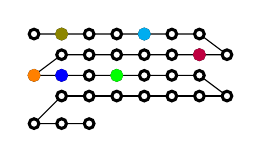
\begin{tikzpicture}[every node/.style={circle, draw, inner sep=2pt, minimum size=6mm}, scale = 0.35, transform shape]
    \tikzstyle{vertex}=[circle, draw = black,fill=White,minimum size=10pt,inner sep=0pt, line width = 1.1 pt]
    
    \foreach \label/\x/\y in {30/1/2.25, 28/2/2.25, 26/3/2.25, 24/4/2.25, 22/5/2.25, 20/6/2.25, 18/7/2.25, 16/8/1.5, 
                     14/7/1.5, 12/6/1.5, 10/5/1.5, 8/4/1.5, 6/3/1.5, 4/2/1.5, 2/1/0.75, 1/2/0.75, 
                     3/3/0.75, 5/4/0.75, 7/5/0.75, 9/6/0.75, 11/7/0.75, 13/8/0, 15/7/0, 17/6/0, 
                     19/5/0, 21/4/0, 23/3/0, 25/2/0, 27/1/-1, 29/2/-1, 31/3/-1}
    \node[vertex] (G-\label) at (\x,\y) {\makebox[0.35cm][c]{}};

    
    \foreach \from/\to in {1/3, 3/5, 5/7, 7/9, 9/11, 11/13, 13/15, 15/17, 17/19, 19/21, 21/23, 23/25, 25/27, 27/29, 29/31, 1/2, 2/4, 4/6, 6/8, 8/10, 10/12, 12/14, 14/16, 16/18, 18/20, 20/22, 22/24, 24/26, 26/28, 28/30}
    \draw (G-\from) -- (G-\to) ;
    \node[vertex, fill = blue, draw = blue] at (G-1) {};
    \node[vertex, fill = orange, draw = orange] at (G-2) {};
    \node[vertex, fill = green, draw = green] at (G-5) {};
    \node[vertex, fill = purple, draw = purple] at (G-14) {};
    \node[vertex, fill = cyan, draw = cyan] at (G-22) {};
    \node[vertex, fill = olive, draw = olive] at (G-28) {};
\end{tikzpicture} \\
\hspace{0.8cm} {Structure A} &
\hspace{0.6cm} {Structure B} & 
\hspace{0.2cm} {Structure C} & 
{Structure D} \\
% Star & 5-nary tree & Binary tree & Chain \\
\end{tabular}